%%%%%%%%%%%%%%%%%%%%%%%%%%%%%%%%%%%%%%%%%%%%%%%%%%%%%%%%%%%%%%%%%%%%%%%%

%%% LaTeX Template for ECAI Papers 
%%% Prepared by Ulle Endriss (version 1.0 of 2023-12-10)

%%% To be used with the ECAI class file ecai.cls.
%%% You also will need a bibliography file (such as mybibfile.bib).

%%%%%%%%%%%%%%%%%%%%%%%%%%%%%%%%%%%%%%%%%%%%%%%%%%%%%%%%%%%%%%%%%%%%%%%%

%%% Start your document with the \documentclass{} command.
%%% Use the first variant for the camera-ready paper.
%%% Use the second variant for submission (for double-blind reviewing).

\documentclass{ecai} 

% \documentclass[doubleblind]{ecai}

%%%%%%%%%%%%%%%%%%%%%%%%%%%%%%%%%%%%%%%%%%%%%%%%%%%%%%%%%%%%%%%%%%%%%%%%

%%% Load any packages you require here. 

\usepackage{latexsym}
\usepackage{amssymb}
\usepackage{amsmath}
\usepackage{amsthm}
\usepackage{booktabs}
% \usepackage{enumitem}
\usepackage{graphicx}
\usepackage{color}

\usepackage[T1]{fontenc}
\usepackage{graphicx}
%\usepackage{color}
%\renewcommand\UrlFont{\color{blue}\rmfamily}

\usepackage{amsmath,amssymb,amsfonts}
\usepackage[inline, shortlabels]{enumitem}
\usepackage{tabularx}
\usepackage{caption}
% \usepackage{titlesec}
\usepackage[english]{babel}
\captionsetup{font=it}
\usepackage{ragged2e}
\usepackage{hyperref}
\usepackage{pifont}
\usepackage{footmisc}
\usepackage{multirow}
\usepackage{algorithm2e}

% --- Tickz
\usepackage{physics}
\usepackage{amsmath}
\usepackage{tikz}
\usepackage{mathdots}
\usepackage{yhmath}
\usepackage{cancel}
\usepackage{color}
\usepackage{siunitx}
\usepackage{array}
\usepackage{multirow}
\usepackage{amssymb}
\usepackage{gensymb}
\usepackage{tabularx}
\usepackage{extarrows}
\usepackage{booktabs}
\usetikzlibrary{fadings}
\usetikzlibrary{patterns}
\usetikzlibrary{shadows.blur}
\usetikzlibrary{shapes}

% ---------

\usepackage{pdfpages}
\usepackage{booktabs}
\usepackage{csquotes}
\usepackage{lipsum}  
\usepackage{arydshln}
\usepackage{float}
\usepackage{smartdiagram}
\usepackage[inkscapeformat=png]{svg}
\usepackage{textcomp}
\usepackage{tabularray}\UseTblrLibrary{varwidth}
\usepackage{xcolor}
\def\BibTeX{{\rm B\kern-.05em{\sc i\kern-.025em b}\kern-.08em
    T\kern-.1667em\lower.7ex\hbox{E}\kern-.125emX}}
% \usepackage{cite}
\usepackage{amsmath}
\newcommand{\probP}{\text{I\kern-0.15em P}}
\usepackage{etoolbox}
\usepackage{listings}
\usepackage{etoolbox}
\patchcmd{\thebibliography}{\section*{\refname}}{}{}{}

%%%%%%%%%%%%%%%%%%%%%%%%%%%%%%%%%%%%%%%%%%%%%%%%%%%%%%%%%%%%%%%%%%%%%%%%

%%% Define any theorem-like environments you require here.

\newtheorem{theorem}{Theorem}
\newtheorem{lemma}[theorem]{Lemma}
\newtheorem{corollary}[theorem]{Corollary}
\newtheorem{proposition}[theorem]{Proposition}
\newtheorem{fact}[theorem]{Fact}
\newtheorem{definition}{Definition}

%%%%%%%%%%%%%%%%%%%%%%%%%%%%%%%%%%%%%%%%%%%%%%%%%%%%%%%%%%%%%%%%%%%%%%%%

%%% Define any new commands you require here.

% \newcommand{\BibTeX}{B\kern-.05em{\sc i\kern-.025em b}\kern-.08em\TeX}

\setlength\tabcolsep{0.5pt}

\newcommand{\before}[1]{\textcolor{red}{#1}}
\newcommand{\after}[1]{\textcolor{green}{#1}}

\newcommand{\old}[1]{\textcolor{orange}{#1}}
\newcommand{\rem}[1]{\textcolor{red}{#1}}
\newcommand{\todo}[1]{\textcolor{orange}{\newline \textit{\textbf{TODO:} #1}} \newline \newline }


\definecolor{codegreen}{rgb}{0,0.6,0}
\definecolor{codegray}{rgb}{0.5,0.5,0.5}
\definecolor{codepurple}{rgb}{0.58,0,0.82}
\definecolor{backcolour}{rgb}{0.95,0.95,0.92}
 
\lstdefinestyle{mystyle}{
    backgroundcolor=\color{backcolour},   
    commentstyle=\color{codegreen},
    keywordstyle=\color{magenta},
    numberstyle=\tiny\color{codegray},
    stringstyle=\color{codepurple},
    basicstyle=\footnotesize,
    breakatwhitespace=false,         
    breaklines=true,                 
    captionpos=b,                    
    keepspaces=true,                 
    numbers=left,                    
    numbersep=5pt,                  
    showspaces=false,                
    showstringspaces=false,
    showtabs=false,                  
    tabsize=2
}
 
\lstset{style=mystyle}


\newcounter{relation}
\setcounter{relation}{0}
\renewcommand{\therelation}{\arabic{relation}}
\newcommand{\relationautorefname}{Relation}

\newenvironment{relation}[1][]{%
    \refstepcounter{relation}%
    \noindent \raggedright \textit{\textbf{Relation. \therelation}} \hfill$}
{%
$ \hfill \phantom{x}

}

\newcounter{proof}
\setcounter{proof}{0}
\renewcommand{\theproof}{\arabic{proof}}
\newcommand{\proofautorefname}{Proof}

\renewenvironment{proof}[1][]{
    \refstepcounter{proof}
    \noindent \raggedright \textit{\textbf{Proof. \theproof}}

    \setlength{\leftskip}{1em}

}
{

\
\setlength{\leftskip}{0pt}
}

%%%%%%%%%%%%%%%%%%%%%%%%%%%%%%%%%%%%%%%%%%%%%%%%%%%%%%%%%%%%%%%%%%%%%%%%

\begin{document}

%%%%%%%%%%%%%%%%%%%%%%%%%%%%%%%%%%%%%%%%%%%%%%%%%%%%%%%%%%%%%%%%%%%%%%%%

\begin{frontmatter}

    \title{Technical Requirements for Demo Setting}

\end{frontmatter}

%%%%%%%%%%%%%%%%%%%%%%%%%%%%%%%%%%%%%%%%%%%%%%%%%%%%%%%%%%%%%%%%%%%%%%%%



\noindent The demo is a Jupyter Notebook. It only requires launching a bash script to install the Jupyter kernel.

\paragraph{Preferred requirements}

\begin{itemize}
    \item The demo should be tested on Ubuntu 22.04 LTS;
    \item The Jupyter Notebook should be opened with Visual Studio Code and optional plugins;
    \item At least 30GB of free space should be available
    \item At least 16GB of RAM should be available
    \item At least 4 CPU cores should be available
\end{itemize}

\paragraph{Steps for setting up the demo}

\begin{enumerate}
    \item Clone Git repo \url{https://github.com/julien6/omarl_experiments} anywhere locally
    \item Open terminal and execute bash file in \textquote{omarl\_experiments \slash tutorial \slash create\_venv.sh}
    \item Open Visual Studio Code and open \textquote{omarl\_experiments \slash tutorial \slash pw\_tutorial.ipynb}
    \item Click on the top-right corner button to select the \textquote{tuto\_env} kernel as shown in \autoref{fig:screenshot_demo}
    \item Execute the first cells for installation of the required packages. You may need to install \textquote{.deb} packages by hand if indicated.
    \item You should be able to execute each cell once.
\end{enumerate}

\begin{figure*}
    \centering
    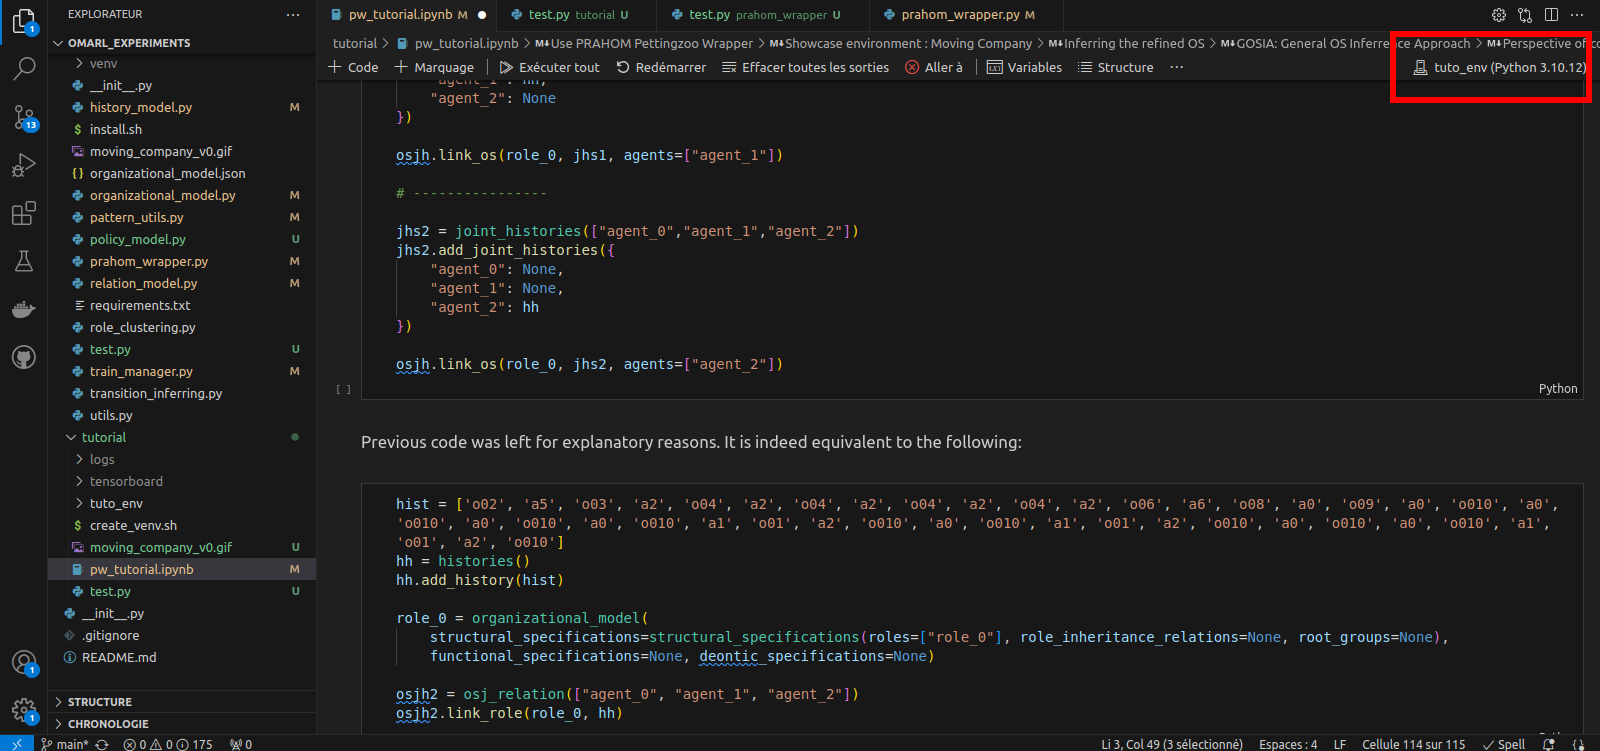
\includegraphics[width=\linewidth]{academic_contributions/Organizational_MARL/ECAI_demo/figures/screenshot_demo.png}
    \caption{Screenshot of the expected demo when configuration done}
    \label{fig:screenshot_demo}
\end{figure*}


\end{document}
%%%%%%%%%%%%%%%%%%%%%%%%%%%%%%%%%%%%%%%%%%%%%%%%%%%%%%%%%%%%%%%%%%%%%%
